\begin{figure}[H]
\label{fig-beamactual}
\caption{The actual behavior of the unbonded beam in bending}
\centering
\vspace{2em}
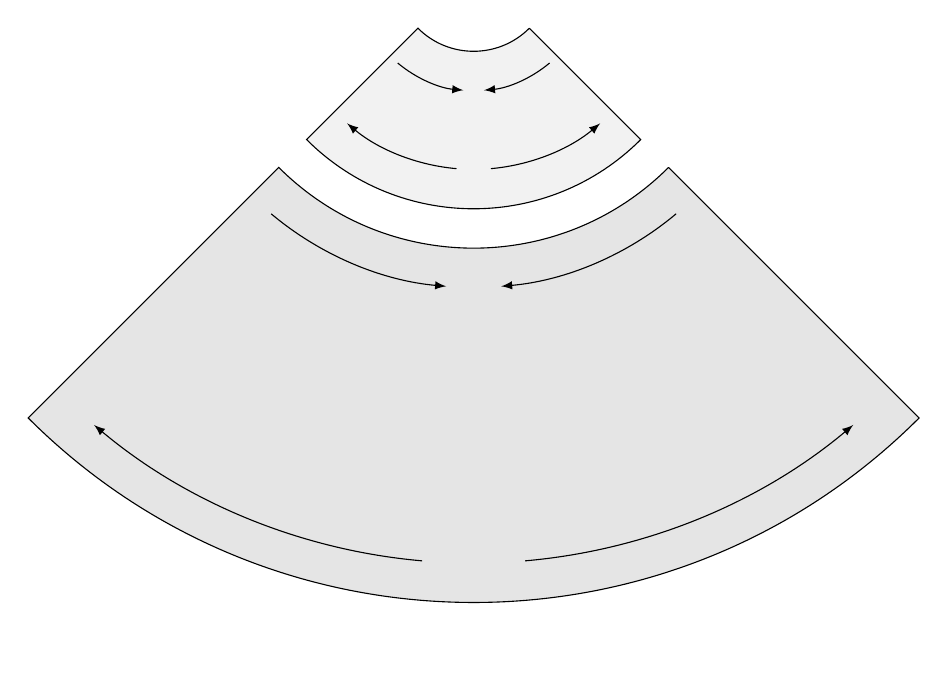
\begin{tikzpicture}[scale=1]
    %\node[] at (0,2) {};
    \draw[fill=gray!10] (-45:1) -- (-45:3) arc(-45:-135:3) -- (-135:1) arc(-135:-45:1);
    \draw[fill=gray!20] (-45:3.5) -- (-45:8) arc(-45:-135:8) -- (-135:3.5) arc(-135:-45:3.5);
    \draw[-latex](-130:1.5) arc (-130:-95:1.5);
    \draw[-latex](-130:4) arc (-130:-95:4);
    \draw[-latex](-50:1.5) arc (-50:-85:1.5);
    \draw[-latex](-50:4) arc (-50:-85:4);
    \draw[-latex](-95:2.5) arc (-95:-130:2.5);
    \draw[-latex](-95:7.5) arc (-95:-130:7.5);
    \draw[-latex](-85:2.5) arc (-85:-50:2.5);
    \draw[-latex](-85:7.5) arc (-85:-50:7.5);
    
\end{tikzpicture}
\end{figure}